\section{算法}
\frame
{
	\frametitle{\secname~ }
	\begin{block}{算法架构}
		算法的基本框架
	\end{block}
	\begin{block}{智能体(策略)更新}
		在固定元参数下的智能体策略更新方式
	\end{block}
	\begin{block}{元学习}
		元参数的学习方式
	\end{block}
}

\subsection*{算法架构}
\frame{
	% \frametitle{总架构}
	\begin{figure}[h]
		\centering
		\includegraphics[width=\textwidth,height=0.28\textwidth]{image/chap03/arch.pdf}
		\caption{网络整体结构图}
		\label{fig:arch}
	\end{figure}
	\vspace{-2em}
	\begin{block}{}
		\footnotesize
		设环境的分布为 $p(\mathcal{E})$ 和智能体的初始参数为 $\theta_0$,则元学习的目标是:
		\begin{equation*}
			\eta^* = \arg \max \mathbb{E}_{\mathcal{E} \thicksim p(\mathcal{E})} \mathbb{E}_{\theta_0 \thicksim p(\theta_0)} [G]
			\label{eq:target}
		\end{equation*}
	\end{block}
}

\subsection*{智能体(策略)更新}
\frame{
	% \frametitle{目标}
	\begin{block}{损失函数}
		智能体策略更新方式就是最小化如下损失函数:
		\footnotesize
		\begin{equation*}
			L(\theta) = \mathbb{E}_{\pi} \left[\sum_t -(G_t - v(s_t) ) \ln \pi_{y_t} (a_t|s_t) + \alpha || (\hat{y}_{t+1}, \hat{G}_{t+1}) - (y_{t+1}, G_{t+1})|| \right]
			\label{eq:agent-update}
		\end{equation*}

	\end{block}
	\begin{block}{策略解析器}
		将 $\pi$ 表示为 $y$ 的线性组合:
		\begin{equation*}
			\pi = \sigma (Wy)
			\label{eq:pred2policy}
		\end{equation*}
		$\sigma$ 是softmax函数
	\end{block}
}

\frame{
	% \frametitle{算法流程}
	\begin{figure}[h]
		\centering
		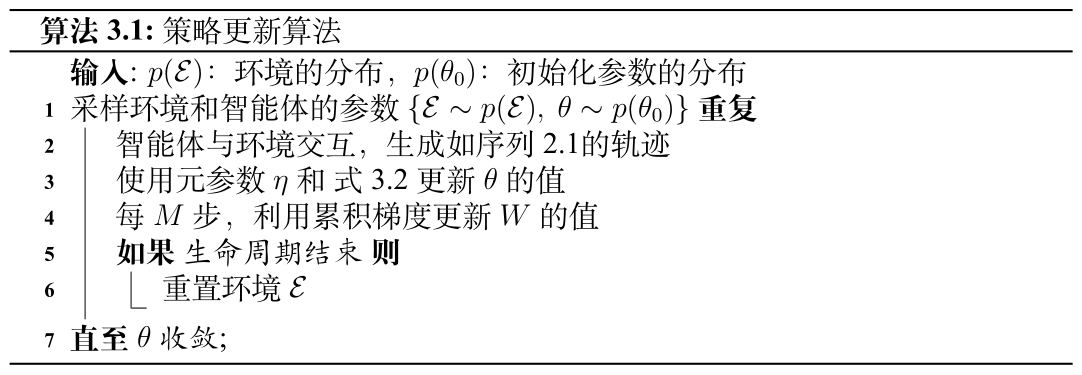
\includegraphics[width=\textwidth]{presentation/figures/alg3_1.png}
		\label{fig:alg3_1}
	\end{figure}
}

\subsection*{元学习}
\frame{
	% \frametitle{更新方式}
	\begin{block}{元梯度}
		元学习的梯度:
		\begin{equation*}
			\Delta \eta  \varpropto \mathbb{E}_{\mathcal{E}} \mathbb{E}_{\theta_0} \left[ \nabla  || (\hat{y}_{t+1}, \hat{G}_{t+1}) - (y_{t+1}, G_{t+1})||  \right]
			\label{eq:meta-gradient}
		\end{equation*}
	\end{block}
}

\frame{
	% \frametitle{算法流程}
	\begin{figure}[h]
		\centering
		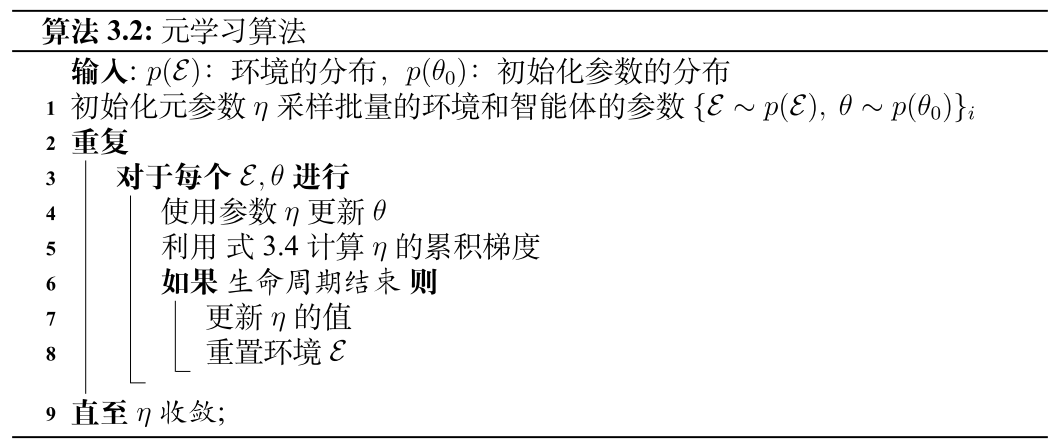
\includegraphics[width=\textwidth]{presentation/figures/alg3_2.png}
		\label{fig:alg3_2}
	\end{figure}
}
